\documentclass{xmgr}
\usepackage{ gensymb }
\usepackage{listings}
\usepackage[table]{xcolor}
\lstset{language=C}
\setcounter{secnumdepth}{5}
\usepackage{paralist}
\definecolor{orange}{rgb}{1,0.5,0}

\makeatletter
\newcommand\footnoteref[1]{\protected@xdef\@thefnmark{\ref{#1}}\@footnotemark}
\makeatother

\author   {Daniel Sienkiewicz}
\nralbumu {206358}
\email    {daniel@sienkiewicz.ovh}


\title    {Projekt komputera samochodowego bazujący na systemie mikrokomputera Intel Galileo}
\date     {2015}
\miejsce  {Gdańsk}

\opiekun  {dr inż. Janusz Młodzianowski}

\begin{document}

\begin{abstract}
Celem pracy jest stworzenie komputera pokładowego do samochodu, w którego skład wchodzi: \begin{enumerate}
\item Mikrokomputer Intel Galileo Gen 1, 
\item Ekran dotykowy FTDI VM800, 
\item Oprogramowanie,
\item Kamerka cofania.
\end{enumerate}

Pierwsza część pracy przedstawia architekturę projektu wraz z jego opisem funkcjonalnym. Opisuję również mechanizmy komunikacji systemu mikroprocesorowego z otoczeniem.

Następnie przedstawiony jest pomysł implementacji oraz proces tworzenia niezbędnej do obsługi symulatora samochodu biblioteki pozwalającej na komunikację z I/O Expanderem PCF8574N.

Ostatnia część pracy przedstawia pomysły  możliwych rozszerzeń projektu o dodatkowe moduły oraz funkcjonalności w zależności od potrzeb użytkownika.
\end{abstract}
\keywords{Intel Galileo, $I^2C$,
 SPI, 
 C, 
 Arduino,
 GPIO,
 FTDI Chip,
 VM800}
\maketitle

%================WPROWADZENIE=====================
\chapter{Wprowadzenie}
\section{Cele}
Celem pracy jest budowa oraz oprogramowanie komputera pokładowego do samochodu. Komputer powinien móc wczytać z czujników temperaturę panującą w silniku, na zewnątrz oraz w środku samochodu. Ponadto powinien on móc zapisać aktualną pozycję GPS na karcie microSD oraz umożliwić korzystanie z kamerki cofania lub inteligentnego lusterka wstecznego.
\section{Założenia}
Do wykonania komputera wykorzystano: Intel Galileo używane w trybie Arduino o oprogramowywane za pomocą Arduino IDE, lokalizator GPS służący do podawania aktualnej pozycji dzięki której obliczana zostaje droga przebyta przez samochód, kamerka internetowa służąca jako czujnik cofania oraz inteligentne lusterko wsteczne oraz symulator samochodu. Aktualnie komputer nie będzie zamontowany do fizycznego samochodu więc do tych celów zbudowany został symulator samochodu składający się z podstawowych czujników takich jak: guziki służące za czujnik zapięcia pasów/zamknięcia drzwi, potencjometry służące za czujniki temperatury oraz I/O expander PCF8574N pozwalający zmniejszyć ilość kabli wychodzących z symulatora do Intel Galileo do 2 zamiast 11. Na komputerze nie będzie wyświetlana aktualna prędkość ani przebieg ponieważ nawet w najnowszych samochodach nie jest to dostępna opcja. Dane te są dostępne na zegarach samochodowych więc nie ma potrzeby powtarzania tej informacji.
\section{Plan pracy}
TO DO
%================KONIEC WPROWADZENIE=====================

%================ARCHITEKTURA=====================
\chapter{Architektura}
\subsection{Opis funkcjonalny}
\subsection{Mechanizmy komunikacji systemu mikroprocesorowego z otoczeniem}
\subsubsection{Porty}

Porty są jednym z najbardziej podstawowych interfejsów. Najczęściej dzieli się je na porty:
\begin{enumerate}
	\item Cyfrowe
	\item Analogowe
\end{enumerate}

Porty cyfrowe charakteryzują się możliwością przyjęcia lub wysłania sygnału binarnego (1 - jest sygnał, 0 - sygnału nie ma). Z kolei porty analogowe mogą przesyłać sygnały nawet 10 bitowe. Każdy z portów może działać w jednym  z dwóch trybów: wejścia - oczekiwać na przyjęcie danych od urządzenia zewnętrznego oraz wyjścia - wysyłać dane do urządzenia zewnętrznego. 


W środowisku Arduino aby obsłużyć port analogowy wystarczy:
\begin{lstlisting}[label=bot-dirs-alg,caption=Obsługa portu analogowego w środowisku Arduino]
int val = 0;
int analogPin = A1;	
pinMode(analogPin, OUTPUT);
val = analogRead(analogPin);
pinMode(analogPin, INPUT);
analogWrite(ledPin, val);
\end{lstlisting}

i odpowiednio dla portu cyfrowego:
\begin{lstlisting}[label=bot-dirs-alg,caption=Obsługa portu cyfrowego w środowisku Arduino]
int val = 0;
int digitalPin = 1;	
pinMode(digitalgPin, OUTPUT);
val = digitalRead(analogPin);
pinMode(digitalPin, INPUT);
digitalWrite(digitalPin, HIGH);
\end{lstlisting}

\subsubsection{Przerwania}

Przerwania są to bezpośrednie funkcje systemu lub sprzętu ułatwiające komunikację ze światem zewnętrznym. Część z nich jest zarezerwowana przez system lecz część z nich jest wolna do wykorzystania dla programisty. Przerwania możemy podzielić na trzy podstawowe rodzaje:

\begin{enumerate}
	\item Programowe
	\item Sprzętowe
	\begin{enumerate}
		\item Maskowalne (NMI)
		\item Niemaskowalne (INTR)
	\end{enumerate}
	\item Wyjątek
\end{enumerate}

Przerwania programowe wywołuje się za pomocą komendy INT XX gdzie XX oznacza numer przerwania zadeklarowanego w tablicy wektorów przerwań, która jest tworzona przy każdorazowym starcie systemu. Przerwanie to może przyjąć wartości do 255 i są one zarezerwowane przez procesor oraz użytkownika.

Przerwanie sprzętowe jest to rodzaj przerwań wywoływanych przez urządzenia wejścia/wyjścia lub zgłaszane przez procesor. Zostają one wywołane niezależnie w określonych przypadkach. Przerwania te dzielimy na maskowalne oraz niemaskowalne. Główna różnica między nimi polega na możliwości zablokowania przerwań maskowalnych podczas gdy przerwania niemaskowalne muszą zostać obsłużone. Przykładem przerwania niemaskowalnego INT2 czyli popularny blue screen of death.

Ostatnim rodzajem przerwań są wyjątki. Wywoływane sa podczas napotkania przez procesor błędów oraz niepowodzeń. Arduino oczywiście obsługuje przerwania. Ich obsłga jets bardzo prosta:
W środowisku Arduino aby obsłużyć port analogowy wystarczy:

\begin{lstlisting}[label=bot-dirs-alg,caption=Obsługa przerwań sprzętowych w środowisku Arduino]
attachInterrupt(pinInt, funcName, mode);
\end{lstlisting}
gdzie pinInt jest to pin na którym Arduino będzie nasłuchiwało na przerwanie, funcName jest to nazwa funkcji który zostanie wykonana gdy przerwanie zostanie zgłoszone, mode - jest to określenie kiedy sygnał może być uznany za przerwanie.

\subsubsection{Odpytywanie w pętli}
Jednym z najprostszych metod pozyskania danych z mikro kontrolera jest jego odpytywanie w nieskończonej pętli.Jest to najmniej efektywny sposób ponieważ cały czas zajmuje niepotrzebnie zasoby sprzętu niepotrzebnymi zapytaniami.

\begin{lstlisting}[label=bot-dirs-alg,caption=Odpytywanie w nieskończonej pętli w środowisku Arduino]
void loop() {
	funcName();
	delay(1000);
}
\end{lstlisting}

\subsubsection{Timer}
\begin{lstlisting}[label=bot-dirs-alg,caption=Użycie timer w środowisku Arduino]
#include <TimerOne.h>
Timer1.initialize(500000); // ustawienie długości timera
Timer1.attachInterrupt(funcName, 500000);
\end{lstlisting}
\subsubsection{Protokół komunikacyjny}
TO DO
\subsubsection{Złączki oraz kable}
TO DO
\subsection{Intel Galileo}
Intel Galileo jest  to mikro kontroler oparty na 32-bitowym procesorze Intel® Quark SoC X1000 i taktowaniu 400MHz. Został on wyposażony w 14 pinów cyfrowych (w tym 6 pinów mogących pełnić funkcję PWM) oraz 6 pinów cyfrowych.Każdy z tych pinów jest w stanie operować napięciem max 5V. Bardzo dużym atutem Galileo jest wbudowana karta sieciowa, port RS-232 oraz port USB oraz slot karty microSD. Galileo może być używane w dwóch trybach - trybie w pełni kompatybilnym z Arduino oraz w trybie z zainstalowanym systemem operacyjnym (np. Linux).

\begin{figure}[!htb]
    \centering
    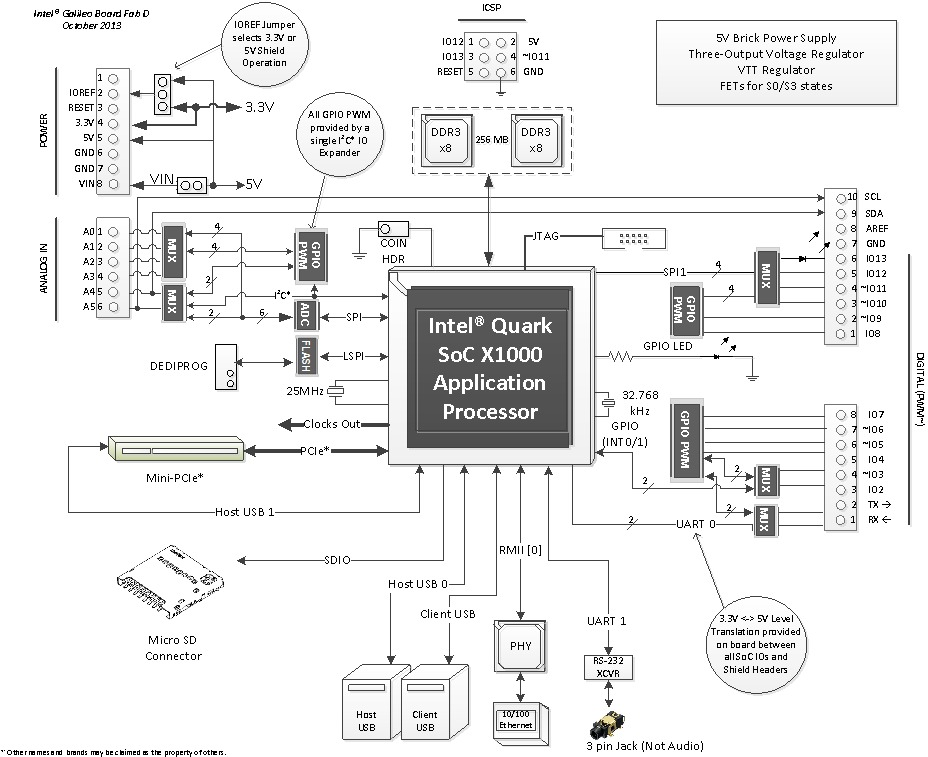
\includegraphics[height=0.3\textheight]{images/IntelGalileoLogicSchematics.jpg}
    \caption{Schemat logiczny układu Intel Galileo\label{IntelGalileoLogicSchematics}}
    \source{\url{https://www.arduino.cc/en/ArduinoCertified/IntelGalileo}}
\end{figure}

ŹRÓDŁO: https://www.arduino.cc/en/ArduinoCertified/IntelGalileo

%================KONIEC ARCHITEKTURA=====================

%================IMPLEMENTACJA=====================
\chapter{Implementacja}
\section{$I^2C$}
\subsection{Problemy z bibliotekami}
\subsection{moja implenatacja $I^2C$ (read)}
\subsection{Schemat blokowy programu}

\begin{figure}[!htb]
    \centering
    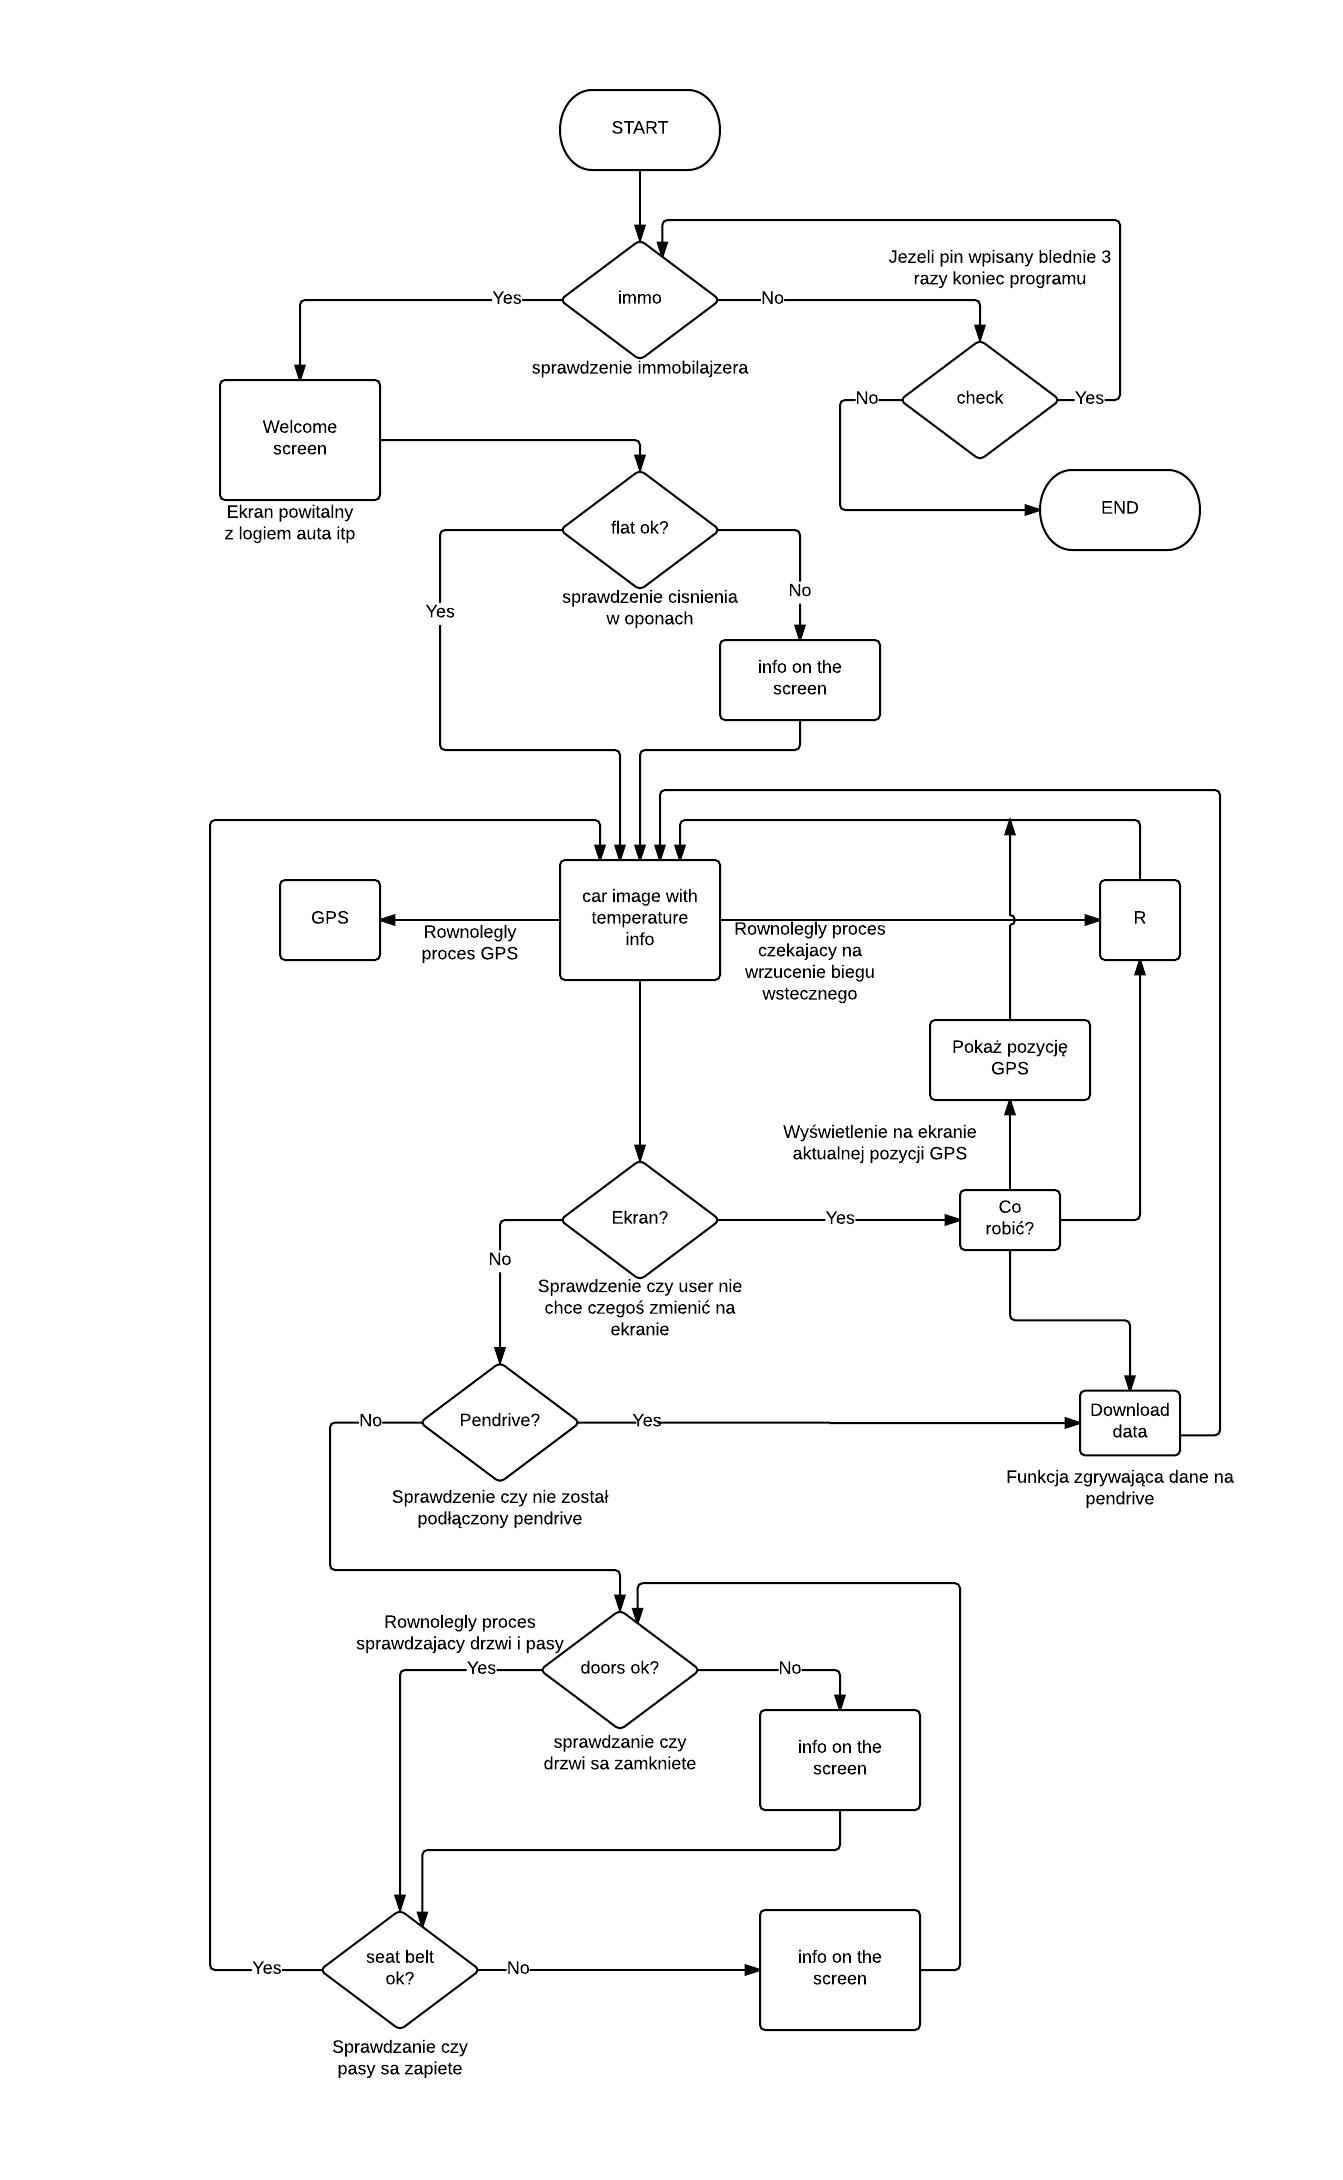
\includegraphics[height=0.4\textheight]{images/schemat_blokowy.png}
    \caption{Schemat blokowy głównego programu\label{SchematBlokowy}}
    \source{Opracowanie własne}
\end{figure}

\subsection{Moja biblioteka do R/W Arduino dla Intel Galileo}
\section{Założenia funkcjonalne}
 - czytanie z czujników, pisanie do ekranu, czytanie z ekranu
 - włączanie i wyłączanie systemu
\section{Integracja z samochodem}
 - podpięcie pod auto
 - włączanie i wyłączanie systemu - można brutalnie wyłączyć
 
 \begin{figure}[!htb]
    \centering
    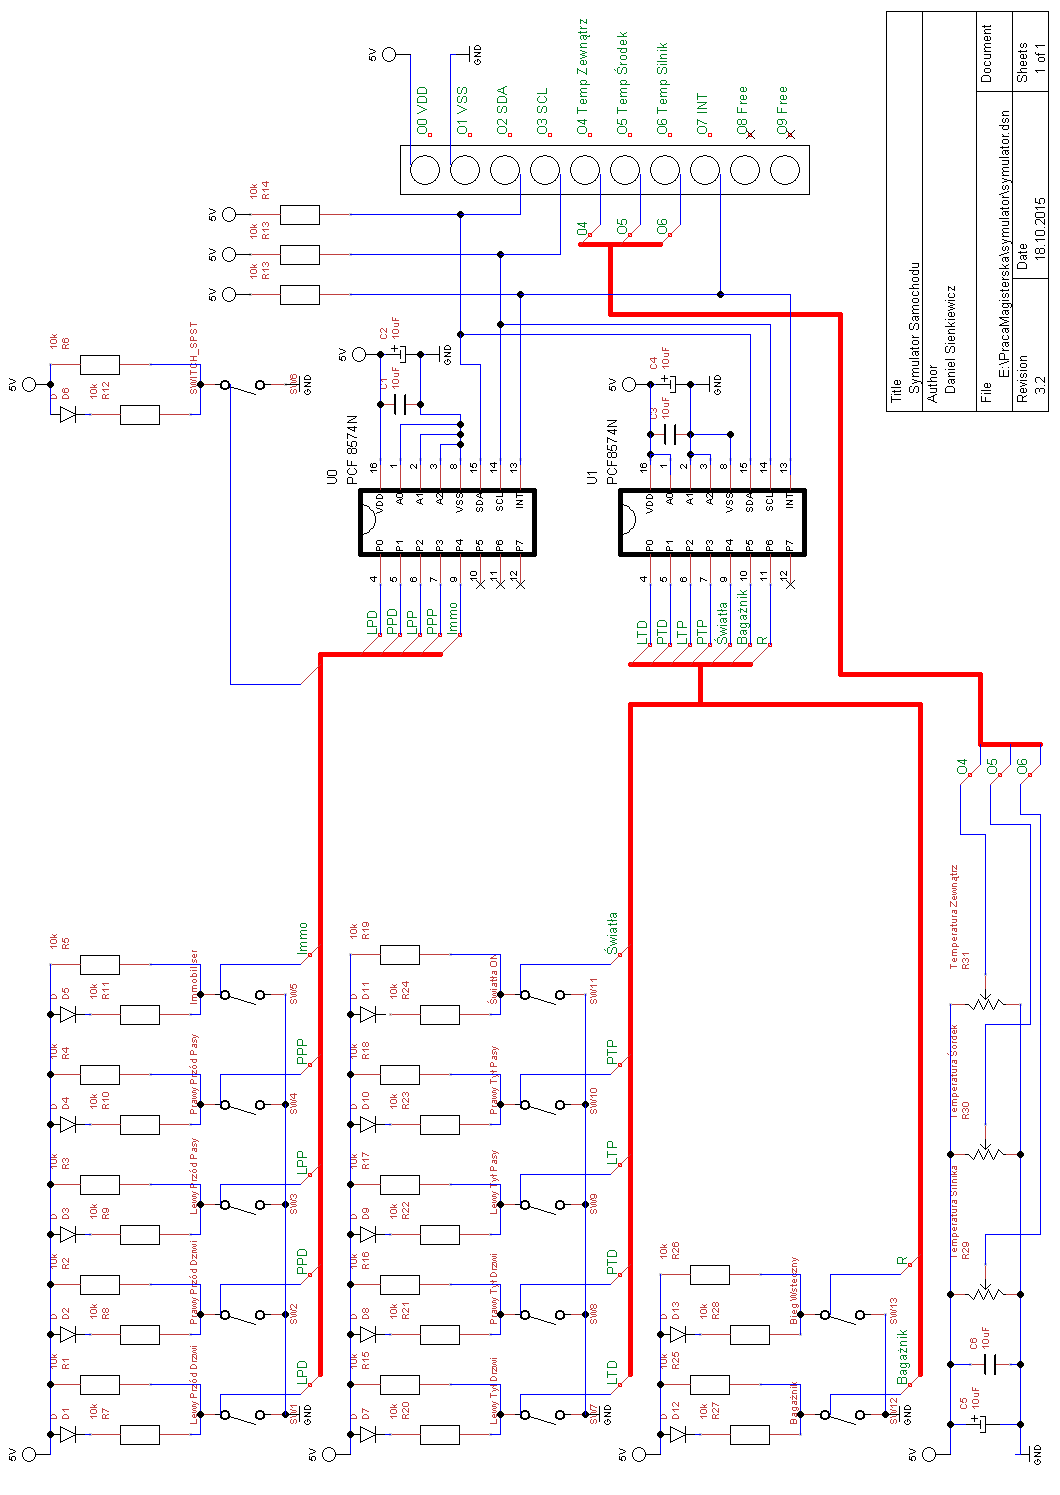
\includegraphics[height=0.4\textheight]{images/symulator.png}
    \caption{Schemat symulatora samochodu\label{SchematSymulatora}}
    \source{Opracowanie własne}
\end{figure}

\section{VM800}
  - na poczatku emulacja na PC
  - potem przepisanie na niski poziom
  - ostatecznie podpiecie do Galielo (poszukac czy juz jest?)
  
   programers manual reference vm800 ftdi POSZUKAĆ!!!!

\section{Dalsze kroki oraz propozycje}
- schemat blokowy z BAJERAMI i wybrane to co zrobię
%================KONIEC IMPLEMENTACJA=====================

\summary
TO DO

\appendix
\chapter{Karty Katalogowe}
Katalog \emph{datasheets} zawiera karty katalogowe użytych podzespołów
\chapter{Porównanie dostępnych na rynku mikro kontrolerów}
\begin{table}[!tbh]
\begin{tabular}{|c|c|c|c|} \hline
 & Intel Galileo & Raspberry Pi (Model B) & Arduino Uno \\ \hline
Wymiary & 10cm x 7cm  & 85.60mm x 56mm x 21mm & 5.59cm x 16.5cm \\ \hline
Procesor & Intel Quark X1000 & Broadcom BCM2835 & ATmega328 \\ \hline
Taktowanie &	400MHz	& 700MHziv & 16 MHz\\ \hline
Cache &	16 KB & 32KB L1 cache, 128KB L2 cache & - \\ \hline
RAM &	512 SRAm & 512 SRAM & 2 kB \\ \hline
Analog I/O	& 6 & 17 & 6 \\ \hline
Digital I/O	& 14 & 8 & 14 \\ \hline
PWM	& 6 & 1 & 6 \\ \hline
\end{tabular}
\caption{Specyfikacja dostępnych na rynku mikro kontrolerów}
\source{\url{http://eu.mouser.com/applications/open-source-hardware-galileo-pi/ http://botland.com.pl/arduino-moduly-glowne/1060-arduino-uno-r3.html}}
\end{table}
\chapter{Programy}
Katalogi \emph{Galileo, PCF8574N} zawierają kod źródłowy oprogramowania stworzonego na potrzeby pracy. 

\noindent Katalog \emph{Galileo} zawiera oprogramowanie mikrokomputera Intel\cite{einstein} Galileo.

\noindent Katalog \emph{PCF8574N} zawiera oprogramowanie I/O Expander PCF8574N.

\bibliographystyle{unsrt}
\bibliography{sample}

\listoftables

\listoffigures

\oswiadczenie

\end{document}